\documentclass{../../../oss-classkick}

\usepackage{circuitikz} % to draw circuits!


\begin{document}
\genheader

\gentitle{1 \& 2}{ELECTROSTATICS}

\genmultidirections

\raggedcolumns
\begin{multicols*}{2}
  
  \begin{enumerate}[leftmargin=18pt]

  \item Two electric objects experience a repulsive force. What happens to that
    force if the distance between the objects is doubled?
    \begin{enumerate}[nosep,leftmargin=18pt,label=(\Alph*)]
    \item It decreases to one-fourth its value.
    \item It decreases to one-half its value.
    \item It stays the same.
    \item It doubles.
    \item It quadruples.
    \end{enumerate}
    \vspace{.7in}
    
  \item A pith ball is a tiny piece of Styrofoam that is covered with a
    conductive paint. One pith ball initially has a charge of \SI{6.4e-8}{C},
    and it touches an identical, neutral pith ball. After the pith balls are
    separated, what is the charge on the pith ball that had the initial charge?
    \begin{enumerate}[nosep,leftmargin=18pt,label=(\Alph*)]
    \item\SI{6.4e-8}{C}
    \item\SI{3.2e-8}{C}
    \item\SI{0}{C}
    \item\SI{-3.2e-8}{C}
    \item\SI{-6.4e-8}{C}
    \end{enumerate}
    \vspace{.7in}
    
  \item Glass becomes positively charged when it is rubbed with silk. Which
    of the following is the best description of what's happening?
    \begin{enumerate}[nosep,leftmargin=18pt,label=(\Alph*)]
    \item Electrons are rubbed off the glass onto the silk.
    \item Electrons are rubbed off the silk onto the glass.
    \item Protons are rubbed off the glass onto the silk.
    \item Protons are rubbed off the silk onto the glass.
    \item Neutrons in the glass have an affinity for positive charge.
    \end{enumerate}
    \vspace{.7in}
    
  \item Consider an isolated, neutral system consisting of wool fabric and a
    rubber rod. If the rubber rod is rubbed with wool to become negatively
    charged, what can be said about the wool fabric?
    \begin{enumerate}[nosep,leftmargin=18pt,label=(\Alph*)]
    \item It becomes equally negatively charged.
    \item It becomes equally positively charged.
    \item It becomes negatively charged but not equally.
    \item It becomes positively charged but not equally.
    \item In a neutral system, neither object can become charged.
    \end{enumerate}
    \vspace{.7in}
    
  \item An electron and a proton are separated by \SI{1.50e-10}{m}. If they are
    released, which one will accelerate at a greater rate, and what is the
    magnitude of that acceleration?
    \begin{enumerate}[nosep,leftmargin=18pt,label=(\Alph*)]
    \item The electron; \SI{1.12e22}{m/s^2}
    \item The proton; \SI{1.12e22}{m/s^2}
    \item The electron; \SI{6.13e18}{m/s^2}
    \item The proton; \SI{6.13e18}{m/s^2}
    \item They both accelerate at the same rate; \SI{1.02e-8}{m/s^2}
    \end{enumerate}
    \vspace{.7in}
    \columnbreak
    
  \item A negatively charged object is placed near, but not touching, a neutral
    conductor. As a result, the two objects are attracted to each other. Which
    of the following is true?
    \begin{enumerate}[nosep,leftmargin=18pt,label=(\Alph*)]
    \item The neutral object gains positive charges to become positively
      charged.
    \item The neutral object loses negative charges to become positively charged.
    \item The neutral object loses positive charges to become negatively
      charged.
    \item The neutral object gains negative charges to become negatively
      charged.
    \item Negative charges of the neutral object move to the side opposite
      the negatively charged object.
    \end{enumerate}
    \vspace{.7in}
    
  \item A rubber comb is rubbed on hair and then attracts paper bits off the
    table. Which of the following best compares the forces on the paper bits?
    \begin{enumerate}[nosep,leftmargin=18pt,label=(\Alph*)]
    \item The gravitational force is stronger than the electric force.
    \item The electric force is stronger than the gravitational force.
    \item The strong nuclear force dominates all other forces.
    \item The normal force is stronger than the electric force.
    \item The magnetic force is stronger than the electric force
    \end{enumerate}
    \vspace{.7in}
    
  \item Which of the following may be said about an object that is a good
    electrical conductor?
    \begin{enumerate}[nosep,leftmargin=18pt,label=(\Alph*)]
    \item The protons are free to move within the object.
    \item The electrons are free to move within the object.
    \item The electrons are bound to their individual atom.
    \item The object cannot maintain its electric charge.
    \item It may be made of materials such as rubber and plastic
    \end{enumerate}
    \vspace{.7in}
    
  \item Paper is considered an insulator. How does a positively charged piece
    of tape pick up a neutral paper bit?
     \begin{enumerate}[nosep,leftmargin=18pt,label=(\Alph*)]
     \item The tape makes the protons flow to the opposite end of the paper,
       causing an attraction between the electrons left behind and the tape.
     \item The tape polarizes the paper atoms, attracting the electrons to the
       side of the atoms closest to the tape.
     \item The tape forces electrons at the opposite end of the paper to flow
       through the paper toward the tape.
     \item The tape polarizes the paper atoms, moving the protons within the
       atoms to the side of the atom farthest from the tape.
     \item It is not possible for a charged object to attract a neutral object.
     \end{enumerate}
     \vspace{.7in}
     \columnbreak
     
   \item Three particles are located on a coordinate system. An electron is
     located at the origin, a proton is located at $(0,1)$, and an electron is
     located at $(1,0)$. What is the direction of the net electrostatic force on
     the electron located at the origin?
     \begin{enumerate}[nosep,leftmargin=18pt,label=(\Alph*)]
     \item To the right on the coordinate plane
     \item At an angle of \ang{45} (up and to the right on the coordinate plane)
     \item Up on the coordinate plane
     \item At an angle of \ang{135} (up and to the left on the coordinate plane)
     \item To the left on the coordinate plane
     \end{enumerate}
     \vspace{.7in}
     
   \item A carbon nucleus has 6 protons. What can be said about the
     electrostatic force between an orbital electron and the carbon nucleus?
     \begin{enumerate}[nosep,leftmargin=18pt,label=(\Alph*)]
     \item The attractive force of the nucleus on the electron is greater than
       the force of the electron on the nucleus.
     \item The attractive force of the nucleus on the electron is less than the
       force of the electron on the nucleus.
     \item The attractive force of the nucleus on the electron is equal to the
       force of the electron on the nucleus.
     \item The repulsive force of the nucleus on the electron is equal to the
       force of the electron on the nucleus.
     \item The repulsive force of the nucleus on the electron is greater than
       the force of the electron on the nucleus.
     \end{enumerate}
     \vspace{.7in}
     
   \item A hydrogen nucleus (charge $+e$) and a beryllium nucleus (charge $+4e$)
     experience a force, $F$. Which of the following expressions may be used
     to solve for the distance between the nuclei?
     \begin{enumerate}[itemsep=4.5pt,leftmargin=18pt,label=(\Alph*)]
     \item$e\sqrt{\dfrac{5k}F}$
     \item$2e\sqrt{\dfrac{k}F}$
     \item$\dfrac{4ke^2}F$
     \item$6Fe^2$
     \item$3Fe^2$
     \end{enumerate}
     \vspace{.7in}
     
   \item Two electrons exert an electrostatic repulsive force on each other. Is
     it possible to arrange the two electrons so the gravitational attraction
     between them is large enough to cancel out the electric repulsive force?
     \begin{enumerate}[nosep,leftmargin=18pt,label=(\Alph*)]
     \item  No, the charge of the electrons squared is much larger than the
       mass of the electrons squared.
     \item No, there is no gravitational force between subatomic particles.
     \item Yes, reducing the radius between the electrons will increase the
       gravitational force as it is proportional to the inverse of the radius
       squared.
     \item Yes, increasing the distance between the electrons will reduce the
       electrostatic repulsion until it is equal to the gravitational force.
     \end{enumerate}
     \vspace{.7in}
     \columnbreak
     
  \item Four charges are arranged at the corners of a square of side a as shown.
    Which of the following is true of the electric field and the electric
    potential at the center of the square?
    \begin{center}
      \begin{tikzpicture}[scale=2]
        \draw[dashed](0,0)--(1,0)--(1,1) node[midway,right]{$a$}--(0,1)--cycle;
        \draw[fill=black](.5,.5) circle(0.03);
        \draw[fill=white](0,0) circle(0.05) node[below left]{$-q$};
        \draw[fill=white](1,0) circle(0.05) node[below right]{$+q$};
        \draw[fill=white](0,1) circle(0.05) node[above left]{$+q$};
        \draw[fill=white](1,1) circle(0.05) node[above right]{$-q$};
      \end{tikzpicture}
    \end{center}
    \begin{tabular}{rcc}
      & \underline{Electric Field} & \underline{Electric Potential}\\
      (A) & zero & zero \\
      (B) & $\dfrac{kQ}{a\sqrt{2}}$ & zero \\
      (C) & $\dfrac{kQ^2}{2a^2}$ &  $\dfrac{kQ}{2a}$\\
      (D) & zero &  $\dfrac{kQ}{\sqrt{2a}}$\\
      (E) & $\dfrac{kQ^2}{2a}$ & $\dfrac{kQ}{a\sqrt{2}}$
    \end{tabular}
    \vspace{.7in}
    
  \item Three charges, $+Q$, $-Q$, and $+2Q$, are arranged in an equilateral
    triangle as shown. Which of the arrows below best represents the direction
    of the electric field at the center of the triangle?
    \begin{center}
      \vspace{-.1in}
      \begin{tikzpicture}[scale=2.2]
        \draw[dashed](0,0)--(1,0)--(.5,.866)--cycle;
        \draw[fill=black](.5,.289) circle(.03);
        \draw[fill=white](0,0) circle(.05) node[left]{$+Q\;$};
        \draw[fill=white](1,0) circle(.05) node[right]{$\;-Q$};
        \draw[fill=white](.5,.866) circle(.05) node[above]{$2Q$};
      \end{tikzpicture}
    \end{center}
    \begin{enumerate}[nosep,leftmargin=18pt,label=(\Alph*)]
    \item $\displaystyle\downarrow$
    \item $\displaystyle\uparrow$
    \item $\displaystyle\searrow$
    \item $\displaystyle\swarrow$
    \item $\displaystyle\nearrow$
    \end{enumerate}
    
  \item Which of the following diagrams best represents how you might rearrange
    the charges so that the electric field at the center would point directly
    toward the top of the page?
    \begin{enumerate}[nosep,leftmargin=18pt,label=(\Alph*)]
    \item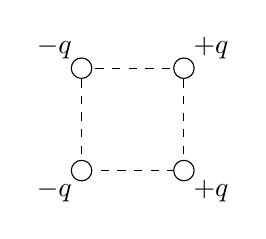
\begin{tikzpicture}[scale=1.3]
      \draw[dashed](0,0) rectangle(1,1);
      \draw[fill=white](0,0) circle(.1) node[below left]{$-q$};
      \draw[fill=white](1,0) circle(.1) node[below right]{$+q$};
      \draw[fill=white](0,1) circle(.1) node[above left]{$-q$};
      \draw[fill=white](1,1) circle(.1) node[above right]{$+q$};
    \end{tikzpicture}
    \item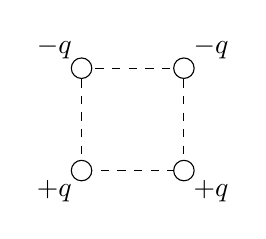
\begin{tikzpicture}[scale=1.3]
      \draw[dashed](0,0) rectangle(1,1);
      \draw[fill=white](0,0) circle(.1) node[below left]{$+q$};
      \draw[fill=white](1,0) circle(.1) node[below right]{$+q$};
      \draw[fill=white](0,1) circle(.1) node[above left]{$-q$};
      \draw[fill=white](1,1) circle(.1) node[above right]{$-q$};
    \end{tikzpicture}
    \item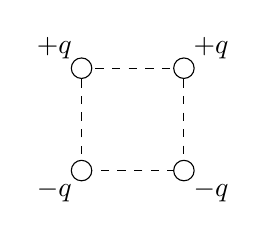
\begin{tikzpicture}[scale=1.3]
      \draw[dashed](0,0) rectangle(1,1);
      \draw[fill=white](0,0) circle(.1) node[below left]{$-q$};
      \draw[fill=white](1,0) circle(.1) node[below right]{$-q$};
      \draw[fill=white](0,1) circle(.1) node[above left]{$+q$};
      \draw[fill=white](1,1) circle(.1) node[above right]{$+q$};
    \end{tikzpicture}
    \item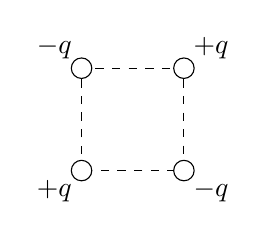
\begin{tikzpicture}[scale=1.3]
      \draw[dashed](0,0) rectangle(1,1);
      \draw[fill=white](0,0) circle(.1) node[below left]{$+q$};
      \draw[fill=white](1,0) circle(.1) node[below right]{$-q$};
      \draw[fill=white](0,1) circle(.1) node[above left]{$-q$};
      \draw[fill=white](1,1) circle(.1) node[above right]{$+q$};
    \end{tikzpicture}
    \item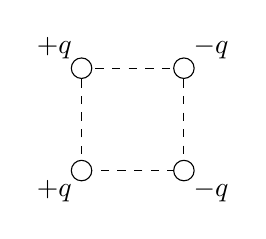
\begin{tikzpicture}[scale=1.3]
      \draw[dashed](0,0) rectangle(1,1);
      \draw[fill=white](0,0) circle(.1) node[below left]{$+q$};
      \draw[fill=white](1,0) circle(.1) node[below right]{$-q$};
      \draw[fill=white](0,1) circle(.1) node[above left]{$+q$};
      \draw[fill=white](1,1) circle(.1) node[above right]{$-q$};
    \end{tikzpicture}
    \end{enumerate}
    \vspace{.7in}
    \columnbreak
    
  \item The electric potential at the surface of the sphere from the last
    question is
    \begin{enumerate}[nosep,leftmargin=18pt,label=(\Alph*)]
    \item $\displaystyle\frac{\beta R^3}{12\epsilon_0}$
    \item $\displaystyle\frac{\beta R}{2\epsilon_0}$
    \item $\displaystyle\frac{\beta R^3}{3\epsilon_0}$
    \item $\displaystyle\frac{\beta R^2}{2\epsilon_0}$
    \item $\displaystyle\frac{\beta R^2}{4\epsilon_0}$
    \end{enumerate}
    
  \item Electric potential
    \begin{enumerate}[nosep,leftmargin=18pt,label=(\Alph*)]
    \item is a vector quantity that depends on the direction of the electric
      field
    \item is a scalar quantity that depends on the magnitude and sign of charges
      in the vicinity
    \item is a scalar quantity that depends on the square of the distance from
      the charges in the vicinity
    \item is a vector quantity that depends on the sign of the charges in the
      vicinity
    \item is a vector quantity that must point from high to low potential
    \end{enumerate}
    \vspace{.7in}
    \columnbreak
    
  \item Which of the following statements is true of electric field and
    equipotential lines?
    \begin{enumerate}[nosep,leftmargin=18pt,label=(\Alph*)]
    \item The electric field vector always points in the same direction as the
      equipotential lines.
    \item The electric field always points in the opposite direction of the
      equipotential lines.
    \item The electric field always points perpendicular to the equipotential
      lines.
    \item The electric field is always equal to the equipotential lines.
    \item Equipotential lines always form a circle around electric field lines.
    \end{enumerate}
  \end{enumerate}
\end{multicols*}
\newpage

\genfreetitle{1 \& 2}{ELECTROSTATICS}{4}

\genfreedirections

\begin{enumerate}

  % FROM TIPLER
\item Two identical small spheres of mass $m$ are suspended from a common point
  by threads of length $L$. When each sphere carries a charge $q$, each thread
  makes an angle $\theta$ with the vertical as shown in the figure below.
  \begin{enumerate}
  \item Express charge $q$ in terms of $\theta$, $m$, $L$ and any other relevant
    constants, and
  \item Compute $q$ if $m=\SI{10}{\gram}$, $L=\SI{50}{\centi\metre}$ and
    $\theta=\ang{10}$.
  \end{enumerate}
  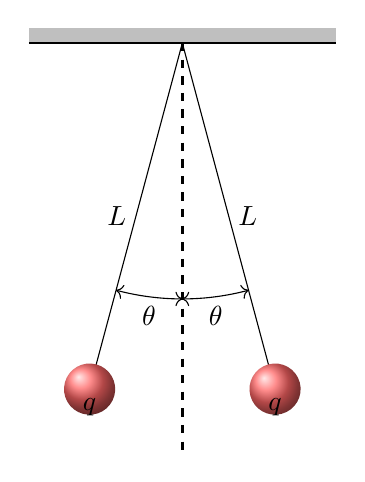
\begin{tikzpicture}[scale=1.3]
    \tikzstyle{balloon}=[ball color=red!60];
    \fill[gray!50](-1.5,0) rectangle(1.5,0.15);
    \draw[thick](-1.5,0)--(1.5,0);
    \draw[dashed,very thick](0,0)--(0,-4);
    \draw[<->](0,-2.5) arc (270:285:2.5) node[midway,below]{$\theta$};
    \draw[<->](0,-2.5) arc (270:255:2.5) node[midway,below]{$\theta$};
    \begin{scope}[rotate=15]
      \draw(0,0)--(0,-3.5) node[midway,right]{$L$};
      \shade[balloon] (0,-3.5) circle (0.25) node[below]{$q$};
    \end{scope}
    \begin{scope}[rotate=-15]
      \draw(0,0)--(0,-3.5) node[midway,left]{$L$};
      \shade[balloon] (0,-3.5) circle (.25) node[below]{$q$};
    \end{scope}
  \end{tikzpicture}
  \newpage
  
  % FROM TIPLER
\item Five equal charges $Q$ are equally spaced on a semicircle or radius $R$
  as shown in the figure below. Find the force on a charge $q$ located at the
  center of the semi-circle. (Hint: Take advantage of symmetry.)
  
  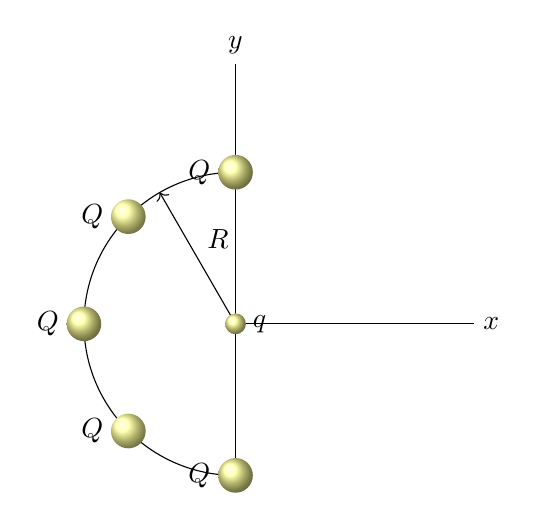
\begin{tikzpicture}[scale=1.1]
    \tikzstyle{balloon}=[ball color=yellow!40];
    \draw(0,-1.75)--(0,3) node[above]{$y$};
    \draw(0,0)--(2.75,0) node[right]{$x$};
    \draw[->,rotate=120](0,0)--(1.75,0) node[midway,above right]{$R$};
    \draw(0,1.75) arc (90:270:1.75);
    \foreach \x in {0,45,...,180}
    \shade[balloon,rotate=\x] (0,1.75) circle (0.2) node[left]{$Q\;\;$};
    \shade[balloon] (0,0) circle(0.12) node[right]{$\;q$};
  \end{tikzpicture}
  \newpage
  
  % THIS IS TAKEN FROM THE 2001 AP PHYSICS B EXAM FREE-RESPONSE QUESTION #3
  \begin{center}
    \begin{tikzpicture}[scale=.8]
      \draw[thick,dashed](0,0)--(4,0) node[midway,below]{$s$}
      --(4,4) node[midway,right]{$s$}--(0,4) node[midway,above]{$s$}
      --(0,0) node[midway,left]{$s$};
      \fill(0,4) circle(.13) node[above left,black]{$+Q$};
      \fill(4,4) circle(.13) node[above right,black]{$-Q$};
      \fill(4,0) circle(.13) node[below right,black]{$+Q$};
      \fill(0,0) circle(.13) node[below right,black]{$-Q$};
    \end{tikzpicture}\\
    Arrangement 1
  \end{center}
  
\item Four charged particles are held fixed at the corners of a square of
  side $s$. All the charges have the same magnitude $Q$, but two are positive
  and two are negative. In Arrangement 1, shown above, charges of the same
  sign are at opposite corners. Express your answers to parts (a) and (b) in
  terms of the given quantities and fundamental constants.
  \begin{enumerate}[leftmargin=15pt]
  \item For Arrangement 1, determine the following.
    \begin{enumerate}
    \item The electrostatic potential at the center of the square
    \item The magnitude of the electric field at the center of the square
    \end{enumerate}
    \begin{center}
      \begin{tikzpicture}[scale=.8]
        \draw[thick,dashed](0,0)--(4,0) node[midway,below]{$s$}
        --(4,4) node[midway,right]{$s$}--(0,4) node[midway,above]{$s$}
        --(0,0) node[midway,left]{$s$};
        \fill(0,4) circle(.13) node[above left,black]{$-Q$};
        \fill(4,4) circle(.13) node[above right,black]{$-Q$};
        \fill(4,0) circle(.13) node[below right,black]{$+Q$};
        \fill(0,0) circle(.13) node[below right,black]{$+Q$};
      \end{tikzpicture}\\
      Arrangement 2
    \end{center}
  \end{enumerate}  
  The bottom two charged particles are now switched to form Arrangement 2,
  shown above, in which the positively charged particles are on the left and
  the negatively charged particles are on the right.
  \begin{enumerate}[resume]
  \item For Arrangement 2, determine the following.
    \begin{enumerate}
    \item The electrostatic potential at the center of the square
    \item The magnitude of the electric field at the center of the square
    \end{enumerate}
  \item In which of the two arrangements would more work be required to remove
    the particle at the upper right corner from its present position to a
    distance a long way away from the arrangement? Justify your answer.
    
    \vspace{.1in}
    \underline{\hspace{.3in}}Arrangement 1\hspace{.5in}
    \underline{\hspace{.3in}}Arrangement 2
    \vspace{\stretch1}
  \end{enumerate}
  \newpage

  % THIS IS TAKEN FROM THE 2005 AP PHYSICS B EXAM FREE-RESPONSE QUESTION #3
  \begin{center}
    \begin{tikzpicture}
      \draw[thick,->](-5,0)--(5,0)
      node[right]{$x$} node[midway,below left]{$O$};
      \draw[thick,->](0,-3)--(0,3) node[above]{$y$};
      \fill(0,-1.5) circle(.1) node[left]{$-a$} node[right]{$+2q$};
      \fill(0, 1.5) circle(.1) node[left]{$a$}  node[right]{$+q$};
    \end{tikzpicture}
  \end{center}
\item Two point charges are fixed on the y-axis at the locations shown in the
  figure above. A charge of $+q$ is located at $y=+a$ and a charge of $+2q$ is
  located at $y=-a$. Express your answers to parts (a) and (b) in terms of $q$,
  $a$, and fundamental constants.
  \begin{enumerate}
  \item Determine the magnitude and direction of the electric field at the
    origin.
  \item Determine the electric potential at the origin.
  \end{enumerate}
  
  A third charge of $-q$ is first placed at an arbitrary point $A$ ($x=-x_0$) on
  the $x$-axis as shown in the figure below.
  \begin{center}
    \begin{tikzpicture}
      \draw[thick,->](-5,0)--(5,0) node[right]{$x$};
      \draw[thick,->](0,-3)--(0,3) node[above]{$y$};
      \fill(0,-1.5) circle(.1) node[left]{$-a$} node[right]{$+2q$};
      \fill(0, 1.5) circle(.1) node[left]{$a$}  node[right]{$+q$};
      \fill(-4,0)   circle(.1) node[below left]{$A$} node[above]{$-q$};
      \draw[|<->](-4,-.3)--(0,-.3) node[midway,fill=white]{$x_0$};
    \end{tikzpicture}
  \end{center}
  \begin{enumerate}[resume]
  \item Write expressions in terms of $q$, $a$, $x_0$, and fundamental
    constants for the magnitudes of the forces on the $-q$ charge at point $A$
    caused by each of the following.
    \begin{enumerate}
    \item The $+q$ charge
    \item The $+2q$ charge
    \end{enumerate}
    
  \item The $-q$ charge can also be placed at other points on the $x$-axis. At
    each of the labeled points ($A$, $B$, and $C$) in the following diagram,
    draw a vector to represent the direction of the net force on the $-q$
    charge due to the other two charges when it is at those points.
    \begin{center}
      \begin{tikzpicture}
        \draw[dashed,->](-5,0)--(5,0) node[right]{$x$};
        \draw[dashed,->](0,-3)--(0,3) node[above]{$y$};
        \fill(0,-1.5) circle(.1) node[left]{$-a$} node[right]{$+2q$};
        \fill(0, 1.5) circle(.1) node[left]{$a$}  node[right]{$+q$};
        \fill(-4,0)   circle(.1) node[below]{$A$};
        \fill (0,0)   circle(.1) node[below left]{$B$};
        \fill(2.5,0)  circle(.1) node[below]{$C$};
      \end{tikzpicture}
    \end{center}
  \end{enumerate}
\end{enumerate}
\end{document}
